\part{PENSAMENTO LEAN}

\chapter[Pensamento Lean]{Pensamento Lean}



\section[Lean na Manufatura]{Lean na Manufatura}

\subsection[Histórico]{Histórico}

Lean é um modo de pensar sobre como entregar valor ao cliente mais rapidamente por meio da eliminação de desperdícios que impedem a qualidade e a produtividade. O Pensamento Lean teve origem no sistema de produção da Toyota (TPS – Toyota Production System) como Lean Manufacturing e surgiu com o objetivo de reduzir desperdícios na produção. É uma filosofia de gestão que promove formas de especificar valor para o cliente, melhora sequência de fluxos de processos, torna o desempenho mais eficiente e elimina desperdícios na produção. 

Para entendermos porque e como surgiu o pensamento Lean é preciso entender o que ele substituiu: a produção em massa.  A produção em massa foi popularizada por Henry Ford. A produção em massa é usada para produzir em larga escala a baixo custo. Ela divide o processo de manufatura em pequenos passos que possam ser desempenhados por trabalhadores com poucas habilidades, para isso é usado um maquinário de alta precisão e um trabalho padronizado. A produção em massa tem uma característica de inflexibilidade, pois alterações na linha de produção podem acarretar alto custo, assim, apenas é econômico produzir grandes quantidades da mesma coisa e da mesma forma (padronização) \cite{hibbs2009}. 

Em 1945, no Japão pós-guerra, o presidente da Toyota Motor Company, Kiichiro Toyoda, desafio sua companhia a se igualar às companhias da América, porque se não a indústria automobilistica Japonesa não sobreviveria. E ficou claro que isso não poderia ser feito adotando o modelo de produção em massa norte-americano, pois no Japão os materiais eram escassos, as encomendas eram inconstantes e havia demanda por variedade, o que impediria o sucesso de produção larga escala de produtos idênticos. 

Taiichi Ohno, chefe de produção da Toyota, notou essas características que inviabilizam a indústria automobilistica japonesa de adotar o modelo de produção em massa. Com isso, Taiichi Ohno experimentou muitas ideias e técnicas que foram inseridas aos poucos no que veio a ser conhecido como Sistema Toyota de Produção. Ele estudou o sistema de produção de Henry Ford e ampliou sua visão como os supermercados norte-americanos controlavam seus estoques. E acrescentou seus conhecimentos de fiação e tecelagem e as percepções dos trabalhodores que ele supervisionava. Ele descreveu o sistema como “um sistema para absoluta eliminação de desperdícios” e explica que o sistema se mantém sobre dois pilares: Just-in-Time (JIT) e Jidoka (autonomação). 

O fluxo Just-in-Time é o único modelo industrial para gerenciar com eficiência a complexidade inerente do custo de se produzir com variedade. Durante muitos anos o Sistema Toyota de produção foi ignorado, até mesmo no Japão, no entanto, após a crise econômica do petróleo nos anos 70, o sistema foi estudado e adotado por outras empresas japonesas devido ao fato de a Toyota ter emergido da crise rapidamente. Após uma década, o Japão passou a ser forte concorrente dos Estados Unidos e da Europa. Com uma investigação, foi descoberto que as empresas japonesas estavam utilizando uma nova abordagem chamada Just-in-Time, que diz respeito ao princípio de eliminar estoques que costuma estarem presentes em produção de larga escala, tendo o foco em fazer tudo em pequenos lotes e estar apto a realizar mudanças de forma rápida. 

O Jidoka surgiu como o mecanismo utilizado pela máquina de tear automática G-Type criada por Kiichiro, ele consiste na paragem automatica da máquina quando um fio quebrava, evitando que ocorressem desperdícios de material ao se produzir produtos defeituosos. Ao eliminar a criação de produtos defeituosos e diminuir desperdícios no processo, a máquina se tornou um sucesso absoluto, melhorando tanto a produtividade quanto a eficiência do trabalho \cite{katayama2010}. Com isso, o conceito que ficou com o Jidoka foi: organizar o trabalho de modo que ele seja imediatamente interropido quando a menor anomalia for detectada, sendo necessário encontrar a causa e a resolução do problema antes de recomeçar a atividade. No português, Jidoka significa autonomoção, que diz respeito ao fato de responder aos eventos de forma instantânea e correta sem ter que ir ao cérebro receber instruções, no caso da máquina assim que surgir um problema ela para \cite{poppendieck}. 

O sistema de produção sofreu alterações ao longo das décadas, nos anos 90 o Pensamento Lean passou a ser o termo usado para descrever este processo desenvolvido e utilizado pela Toyota. Assim, o Sistema Toyota de Produção, baseado no que hoje é chamado de Pensamento Lean, começou a ser formado nos anos 50 e aos poucos os resultados puderam ser notados na indústria automobilistica mundial. Como a figura 4 mostra nos anos 50 a Toyota nem sequer aparecia do ranking de vendas liderado pela GM e pela Ford. Já nos anos 70 o cenário começou a mudar, a Toyota passou a aparecer na sexta posição do ranking e teve uma ascendência até 2007 onde se tornou líder do ranking de vendas.

\begin{figure}[h]
		\centering
		\label{fig01}
			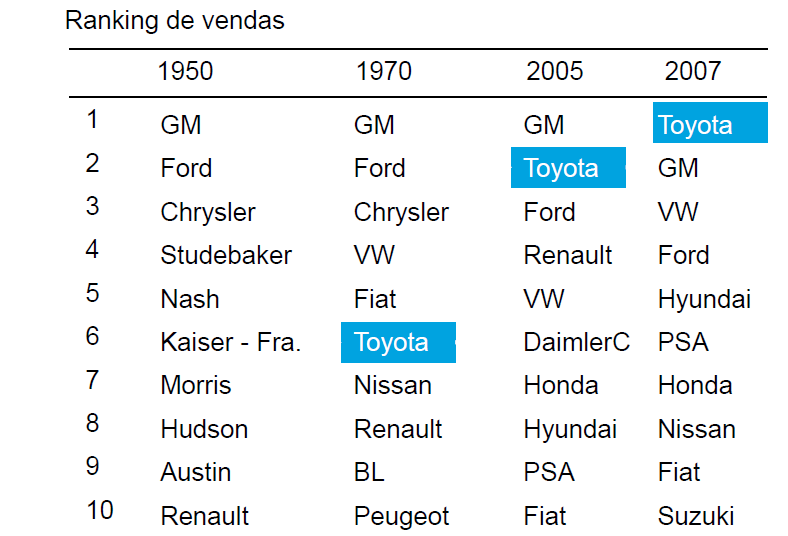
\includegraphics[scale=0.5]{figuras/ranking.png}
		\caption{Ranking de Vendas da Indústria Automobilística  \cite{ranking}}
\end{figure}

\subsection[Princípios]{Princípios}

O Pensamento tem como objetivo fornecer o que o cliente deseja sem haver desperdícios. Para atingir este objetivo Lean possui alguns princípios. Muitas companhias e indivíduos que querem implementar o Pensamento Lean cometem o erro de ficarem preocupados e focados em especificar ferramentas e práticas. Quando aplicadas de forma correta, as ferramentas podem gerar bons resultados de desempenho, mas são os princípios inseridos na cultura da organização que resultarão na mudança de comportamento em longo prazo. Sem uma clara compreensão dos princípios que regem o Pensamento Lean, as empresas conseguirão resultados a curto prazo, mas a longo prazo não consiguiram manter esses bons resultados e a melhoria contínua que irão dar estabilidade ao negocio e à satisfação do cliente. Assim, é preciso enfativar os princípios acima das ferramentas. Os princípios do Pensamento Lean são apresentados na figura 5 e serão descritos nas seções a seguir.

\begin{figure}[h]
		\centering
		\label{fig02}
			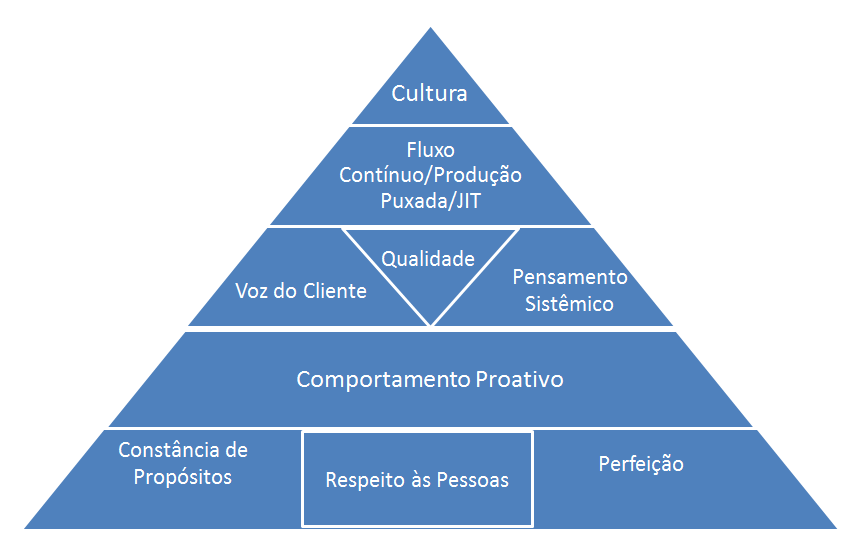
\includegraphics[scale=0.7]{figuras/principioslean.png}
		\caption{Pirâmide de Princípios Lean}
\end{figure}

\subsubsection[Constância de Propósitos]{Constância de Propósitos}

O princípio de Constância de Propósitos diz respeito a manter a clareza dos objetivos importantes de longo prazo e é um dos constituintes da base da pirâmide dos princípios porque prover a persistência necessária para influenciar o comportamento de todos dentro da organização. Quando diariamente o comportamento muda, a cultura da organização também muda. A Constância de Propósitos tem o foco no pensamento e no comportamento, alinhando esforçando e fazendo com que todos caminhem na mesma direção. As pessoas devem ser encorajadas a desafiar o modo como as coisas são feitas e começar a perceber dificuldades e oportunidades de melhoria, resolução de problemas de forma colaborativa e propriedade do processo de qualidade começam a nascer \cite{bell2011}.

Com isso, líderes executivos têm a responsabilidade de definir objetivos estratégicos e criar constância de propósitos. Os gestores tem como responsabilidade eliminar impedimentos, estabilizar os processos e ajudar os trabalhadores a desenvolver habilidades de resolução de problemas, para que eles possam sentir-se donos do seu trabalho e possam assumir responsabilidade sobre a melhoria contínua. 


\subsubsection[Respeito às Pessoas]{Respeito às Pessoas}

O segudo princípio base é o respeito às pessoas. Todos os indivíduos possuem uma única coleção de experiências e fazem distintas contribuições quando participam de um processo de melhoria. A resolução de problemas coletiva só ocorre quando existe respeito pelas pessoas em todos os níveis hierárquicos de uma organização. Respeito direciona desenvolvimento dos trabalhadores, encoraja participação e melhora a relação entre fornecedor e cliente \cite{bell2011}.

Além disso, respeito às pessoas encoraja alcançar a excelência profissiona e o pontêncial criativo. Em um ambiente de aprendizado e desenvolvimento colaborativo as pessoas sabem que suas ideias possuem valor e são apreciadas, e sentem-se mais estimuladas em melhorar diariamente. Pessoas estimuladas e respeitadas não só geram sucesso individual como também sucesso coletivo e organizacional.


\subsubsection[Melhoria Contínua e Perfeição]{Melhoria Contínua e Perfeição}

O último princípio da base da pirâmide é a melhoria contínua em busca da perfeição.  As soluções imediadas, emboram possam ser adequadas para hoje, são na melhor das hipoteses temporárias.  A mudança é constante, e novas ideias são necessárias  sempre que o padrão de trabalho atual não produz mais os resultados esperados. Em uma cultura Lean, os trabalhadores devem aceitar as mudanças como inevitáveis e de forma proativa enfrentar os desafios. Cada indivíduo deve ver o seu trabalho como tendo dois componentes inseparáveis: trabalho diário e melhoria diária \cite{bell2011}.

As pessoas possuem hábitos diferentes. Muitas pessoas gostam da mudança, mas não gostam de serem mudadas. Mudança efetiva costuma ser inconfortável.  Com isso, as pessoas costumam resistir a mudanças e impedir que a criatividade e inovação sejam desenvolvidas dentro de si.  Quando Lean é visto como um programa ou projeto, com início e fim, elas costumam aceitar e realizar o que é pedido. Quando o programa termina, voltam a praticar os mesmo hábitos e comportamentos de antes.

Quando coletivamente as pessoas reconhecem que se não estão melhorando, estão ficando para trás, a compreenssão do trabalho diário muda radicalmente. Esta percepção inspira novas ideias e a reinvenção diária influenciando no sucesso de toda a organização. Com foco constante em melhoria evita-se cair na estagnação no comportamento diário de cada um.


\subsubsection[Comportamento Proativo]{Comportamento Proativo}

O princípio que fica sobre a base da pirâmide é o de comportamento proativo, que significa tomar iniciativa, assumindo pessoal responsabilidade pela qualidade do próprio trabalho e pelo ambiente de trabalho. Ser proativo significa aproveitar a oportunidade para fazer a diferença dia a dia \cite{bell2011}.

Em os 7 Hábitos de Pessoas Altamente Eficazes, o Dr. Stephen Covey introduz um modelo chamado Matriz de Gerenciamento de Tempo, dividindo o trabalho em quatro quadrantes com base na importância e urgência, como ilustrado na figura 6.

\begin{figure}[h]
		\centering
		\label{fig03}
			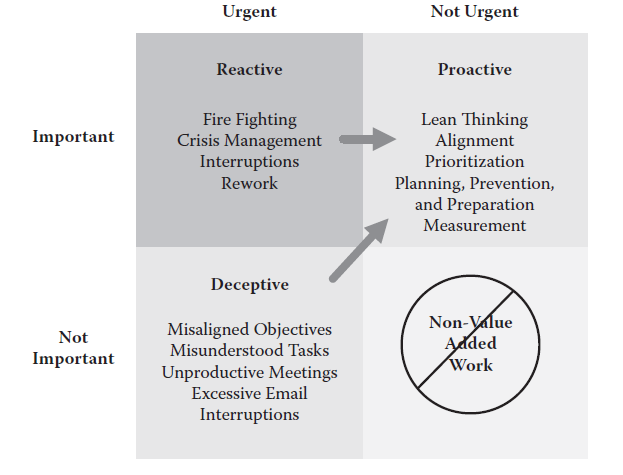
\includegraphics[scale=0.9]{figuras/matrizcomportamento.png}
		\caption{Matriz de Gerenciamento de Tempo \cite{bell2011}}
\end{figure}

Ele ressalta que o trabalho de maior valor encontra-se no quandrante importante e não urgente, onde o planejamento proativo, a prevenção, a preparação e a aprendizagem serão mais fortemente desenvolvidos. Trabalho não planejado concentra-se no quadrante importante e urgente (combate de forma reativa) ou não importante e urgente (atividades que parecem importante devido à sua urgência). Em ambos os casos, eles roubam tempo e recursos que devem ser usados para abordar proativamente o trabalho importante e não urgente. O comportamento reatiavo, geralmente, deixa desperdício e impede o progresso. 

Lean desloca-se da ênfase em sempre realizar trabalho não planejado para o trabalho proativo de melhoria contínua. Esta é uma abordagem eficaz porque quanto mais tempo é gasto na melhoria contínua, menos trabalho não planejado e urgente aparecem e mais tempo é liberado para trabalhar de forma proativa.

O próximo nível da pirâmide está relacionado ao conhecimento em três perspectivas: voz do cliente, qualidade na raíz e pensamento sistêmico.

\subsubsection[Voz do Cliente]{Voz do Cliente}

A maioria dos processos têm tanto os clientes internos que irão receber os produtos de trabalho e o rendimento deles quanto os clientes externos (parceiros comerciais e usuários finais) que rebem o produto final, serviço ou informação. Para compreender claramente a voz do cliente é preciso estar envolvido com os clientes, seja ele quem for \cite{bell2011}.

Use a segmentação de clientes, entrevistas, grupos focais, pesquisas, análises de dados e observação para desenvolver e perceber quais são os requisitos de qualidade críticos. Em seguida, é necessário encontrar regurlamente o cliente para garantir melhorias e inovações e entregar o que o cliente mais valoriza.

Assim, constantemente ouvir a voz do cliente garante que você está focado nas questões certas e fazendo melhorias que serão valiosas para os clientes atuais e futuros. Entender as necessidades e desejos dos clientes mais claramente que seu concorrente faz com que seja mais competitivo e ágil.

\subsubsection[Qualidade na Raíz]{Qualidade na Raíz}

A qualidade na raíz significa fazer as coisas certas da primeira vez sempre, trabalho com problemas ou imperfeito não é enviado para etapa seguinte ou para o cliente. A abordagem de concertar mais tarde um problema é praticado em muitas organizações devido a pressão do prazo, inadequado treinamento e conhecimento não adequado do processo.  A melhor hora de resolver um problema é quando ele acontece porque a causa ainda está fresca, os trabalhadores estão atentos e isso previne a adição de defeitos até que a causa do problema seja encontrada.  O foco do trabalho diário deve ser produzir qualidade desde o início. Correções demoradas e esclarecimentos tornam-se necessárias quando a qualidade é pobre, criando interrupções e atrasos que aumentam os custos e aborrecimentos \cite{bell2011}.

Em um ambiente Lean existe a obrigação de parar e corrigir problemas e um comprometimento coletivo de não deixar que os defeitos conhecidos cheguem até o cliente. Por meio do trabalho padronizado e do treinamento todo esforço é feito para garantir que o problema ou defeito seja repetido novamente. As pessoas assumem a responsabilidade do trabalho que elas passam adiante, independentemente de onde veio o problema. Essa mudança fundamental na atitude reduz o desperdício e a frustração. Com isso, quando a qualidade na raíz toma conta, mais tempo é disponibilizado para desenvolver o que o cliente está pagando, o que por sua vez melhora a produtividade, custo, qualidade e moral.

\subsubsection[Pensamento Sistêmico]{Pensamento Sistêmico}

O terceiro elemento do terceiro nível da pirâmide é o pensamento sistêmico: a capacidade de visualizar a interligação entre os processos que compõesm a cadeia de valor inteira embora esteja ciente da interdependência de causa e efeito que podem criar valor ou criar desperdícios \cite{bell2011}.

A cadeia de valor é composta de todos os processos, atividades e tarefas usados para gerar um produto ou serviço desde a sua concepção até a sua entrega ao cliente, e inclui todas as informações, procedimentos e materiais. Para evitar soluções que criem otimização localizada, o Pensamento Lean requer conhecimento da natureza da simultaneamente integrada e interdependente  de todas as regras de negócio e fluxos de informações.   

Esta não é a forma natural que a mente humana e as organizações trabalham, as pessoas tendem a concentrar-se em partes espcíficas de um quebra-cabeça em vez de concentrar-se em toda a imagem. Medidas inadequadas e os incentivos muitas vezes reforçam essa estreita forma de concentrar.

Quando a solução de problemas baseia-se em uma compreensão clara da cadeia de valor global e os clientes que são atendidos por ela, as empresas evitam o erro comum de realizar melhorias locais, que muitas vezes transferem ineficiências e desperdícios de uma área para a outra. Equipes multifuncionais fornecem a amplitude de entendimento necessário para o pensamento sistêmico, abrangendo o fluxo de valor, ligando o conhecimento e a compreensão de cada membro da equipe.

A perspectiva holística mostrada aqui pode ser desconhecida para muitos profissionais que passaram suas carreiras a aperfeiçoar as habilidades em uma área especializada da empresa. Um pensamento sistêmico estimula o potencial criativo dos trabalhadores, ampliando seus horizontes e desafiando a amplitude de sua percepção. Para fazer melhorias que impactam no que é recebido pelo cliente externo, a cadeia de valor deve ser vista como um sistema. O mapeamento do fluxo de valor e o pensamento sistêmico são complementares, ambos ajudam as pessoas a ver processos de negócios em um novo contexto: fluxo. Assim, o pensamento sistêmico permite ver o todo, criando um fluxo de valor para o cliente.

\subsubsection[Fluxo Contínuo, Produção Puxada e Just in Time]{Fluxo Contínuo, Produção Puxada e Just in Time}

O próximo nível da pirâmide concentra-se no fluxo: a progressão ininterrupta de materiais, serviços e informações.  Como Jeffrey Liker enfatiza no “Toyota Way”: permitir que o trabalho flua sempre que puder, quando o fluxo é interrompido, utilize sinais para puxar o início do trabalho.

O fluxo é conseguido por meio da eliminação de atrasos e interrupções durante toda a cadeia de valor. O mapeamento do fluxo de valor é uma ferramenta eficaz para identificar, quantificar e eliminar o desperdício. O fluxo de informações produz a transparência e visibilidade necessária para coordenar de forma eficiente o fluxo de trabalho. Quando a informação é usada para nivelar a demanda, equilibrar a capacidade e melhorar a qualidade, o fluxo é melhorado e valor é entregue ao cliente de forma rápida. 

Quando não há interrupções em uma série de tarefas, o trabalho flui sem problemas. Tipicamente, o trabalho irá fluir até encontrar uma barreira que impeça sua continuidade, por exemplo, o 
transporte para o outro local. 

A produção puxada diz respeito a o cliente puxar a cadeia de valor. Ou seja, o cliente determina qual é o produto que ele deseja. Com isso, a produção é feita sobre demanda, a produção em massa deve ser eliminada, pois ela empurra o produto para o cliente sem que ele tenha oportunidade de decidir o que é de valor para ele. Assim, a produção puxada inverte o valor produtivo: as empresas não mais empurram os produtos para o consumidor por meio de descontos e promoções. O consumido que passa a “puxar o fluxo do valor”, reduzindo estoques e valorizando o produto.

O Just in Time como dito na seção anterior é um dos pilares do Pensamento Lean e estar relacionado aos dois conceitos anteriores. Ele tem como objetivo eliminar todas as fontes de desperdício e tudo o que não acrescenta valor à organização. O princípio para atingir este fim é simples: só produzir o que é pedido pelo cliente e só quando ele o pretende, ou seja, não manter estoques, seja de produtos acabados ou intermediários. 

\subsubsection[Cultura]{Cultura}

O princípio topo da pirâmide é a cultura, que representa crenças compartilhadas de uma organização e os valor, que se manifestam como atitude e comportamento. Cultura é o resultado da mudança de comportamento. A cultura Lean de melhoria contínua cria uma capacidade compartilhada que permite que as pessoas busquem ser proativas e resolvam problemas, resultando em um desempenho superior, vantagem competitiva e bons resultados financeiros \cite{bell2011}.

A evolução de uma cultura Lean geralmente começa com adoção de práticas de melhoria contínua, seguido pela formação de um comportamento orientado a sistemas e orientado por valores e princípios comuns. As ferramentas fornecem estrutura e capacitação. Sistemas desenvolvem práticas em comum. E princípios fornecem a base que reforça os padrões culturais e o comportamento diário.

\subsection[Conceitos de Valor e Desperdício]{Conceitos de Valor e Desperdício}

O principal foco do Lean é a resolução de problemas com o propósito de entregar valor ao cliente, com base na sistemática eliminação de desperdícios ao longo do fluxo ou cadeia de valor. Portanto, esses três conceitos: valor, fluxo de valor e desperdícios precisam estar claros.

Para um entendimento mais conciso do Pensamento Lean é importante ainda ter em mente que o termo desperdício recebe uma conotação específica e uma autêntica subordinação à ideia de valor. Ou mais especificamente, ao valor percebido pelos clientes considerando suas expectativas, necessidades e desejos. A melhor maneira para se identificar os desperdícios segundo o pensamento Lean, é você se colocar na posição do seu cliente e refletir criticamente sobre os processos de produção, na forma como são realmente feitos \cite{costa2010}.

\subsubsection[Valor]{Valor}

O ponto de partida para o Pensamento Lean consiste em definir o que é valor e o fluxo do valor. Diferente do que muitos pensam, não é a empresa, e sim o cliente quem define o que é valor. Para ele, a necessidade gera o valor, e cabe às empresas determinarem qual é essa necessidade, procurando satisfazê-la e cobrar um preço específico, a fim de manter a empresa no negócio e aumentar seus lucros por meio de melhoria contínua dos processos e da qualidade \cite{leaninstitute}. Assim, valor é aquilo que o cliente deseja e pelo que ele paga. 

\subsubsection[Cadeia de Valor]{Cadeia de Valor}

O fluxo de valor é composto por todo o ciclo de vida dos processos requeridos para gerar serviços, produtos e informação do conceito ao cliente.  Isto incluí todas as atividades, que criam ou não valor. O pensamento sistêmico ajuda as pessoas a perceberem o processo e entender o valor da perspectiva do cliente. 

Para isso, é preciso dissecar a cadeia produtiva e separar os processos em três tipos: os que efetivamente geram valor, aqueles que não geram valor, mas são importantes para a manutenção do processo e para a qualidade do processo e do produto, e aqueles que não agregam valor e que devem ser eliminados, ou seja, os desperdícios \cite{leaninstitute}.

\subsubsection[Os Três Ms]{Os Três Ms}

De acordo com o Lean, os desperdícios podem ser divididos em três categorias, conhecidas como os três Ms: mura, muri e muda. O Mura significa irregularidade e variação, ele representa a inconsistência no fluxo de trabalho, causada pelas mudanças, variedade e qualidade desejadas pelo cliente. É preciso saber minimizar os impactos causados pelo mura por meio da padronização do processo. 

O Muri significa sobrecarga, que representa a carga excessiva sobre as pessoas ou sobre os equipamentos, o que pode causar stress, erros e retrabalho. É preciso saber remover sobrecargas por meio da padronização do processo e gerenciamento adequado da demanda. E o Muda diz respeito ao desperdício em si, que na produção da Toyota foram identificados sete: superprodução, estoque, tempo de espera, transporte, processos inadequados, movimentação de pessoas e correção devido à defeitos.

\subsection[Práticas e Ferramentas]{Práticas e Ferramentas}

O Pensamento Lean sugere um conjunto de práticas e ferramentas que podem ser aplicadas na organização a fim de atingir os objetivos por defendidos por ele. Vale ressaltar que as práticas aqui apresentada são as consideradas principais, a organização deve buscar aqueles que melhor se adeque ao seu contexto. Como dito anteriormente, as ferramentas servem de estrutura e meio de capacitação, é importante que os trabalhadores, sobretudo, vivam diariamente os princípios da cultura Lean.

\subsubsection[A3 Thinking]{A3 Thinking}

O pensamento A3 é a aplicação consistente do PDCA(Plan, Do, Check and Act) na resolução de problemas para identificar o melhor caminho para enfrentar desafios e oportunidades. O pensamento A3 guia as atividades da equipe em direção a uma correta definição dos problemas ou oportunidades. A ferramenta usada no pensamento A3 é o relatório A3, que se refere a um formato padronizado de comunicação que expressa o processo de resolução de problema em uma folha de papel em tamanho A3.

O uso de apenas uma folha para expressar todo o conhecimento faz com que as pessoas refinem seus pensamentos de modo que todas as questões e soluções sejam expostas de forma simples \cite{liker}. 

\subsubsection[Mapeamento da Cadeia de Valor]{Mapeamento da Cadeia de Valor}

O mapeamento da cadeia de valor é uma das ferramentas mais utilizados no Lean, ele permite identificar todas as atividades de um processo da organização que criam ou não criam valor do ponto de vista do cliente, ou seja, permite visualizar todo o fluxo, ao longo da cadeia de valor, desde a conceituação até à entrega ao cliente \cite{bell2011}.

O mapeamento do fluxo de valor representa visualmente o fluxo de informações e materiais com ênfase na quantificação de desperdícios e na quantificação de tempo e qualidade. Ele pode ser feito com grande nível de detalhe, porém, tipicamente, o foco está em um nível mais macro do que no mapeamento de processos  e não inclui tarefas e decisões individuais.

\subsubsection[Kaizen]{Kaizen}

O Kaizen é uma das práticas sugeridas pelo Lean. A palavra Kaizen é a junção de duas palavras japonesas: Kai que significa mudança e Zen que significa bom, porém é comum traduzi-la para melhoria contínua. O Kaizen  pode ser considerado uma forma de atingir os objetivos do Lean \cite{bell2011}.

Esta melhoria é obtida por todos os trabalhadores focando os esforços na eliminação de todo tipo de desperdício. Apesar de este ser um processo lento e incremental, os ganhos em longo prazo são grandes.

Um dos conceitos utilizados pelo Kaizen é o PDCA, desenvolvido por William Edwards Deming, que é orientado à resolução de problemas, este ciclo enfatiza a prevenção de problemas por meio da padronização em busca da melhoria contínua. 

Esta metodologia é composta por quatro etapas:
\begin{itemize}
\item Planejar, que é onde é feita a definição do problema, bem como suas possíveis causas e soluções, o estabelecimento de um plano corretivo e os objetivos de forma clara;
\item Fazer, que é onde o plano é implementado e os dados são recolhidos para análise;
\item Verificar, que é onde é verificado se os dados recolhidos vão de encontro aos objetivos definidos e é feito o registro dos resultados;
\item Agir, que é onde são padronizados os resultados que foram eficazes e se houver medidas não eficazes, o ciclo e refeito.
\end{itemize}

Assim, o Kaizen é um processo incremental e contínuo, que abrange toda a organização e o envolvimento de todos os trabalhadores. Todos devem trabalhar de forma proativa em busca da melhoria diária e acreditar que bons resultados virão em longo prazo.

\subsubsection[Metodologia 5S]{Metodologia 5S}

Os 5S pode ser considerada a ferramenta mais básica que o Lean sugere, é considerado um passo a mais em direção à melhoria da qualidade e da produtividade. O objetivo desta prática é organizar o ambiente de trabalho de forma adequada para que o trabalhador tenha, apenas, os materiais e ferramentas necessários para executar seu trabalho a sua disposição de forma rápida \cite{bell2011}. 

O nome desta metodologia é originado de cinco palavras japonesas: Seiri, Seiton Seiso, Seiketsu e Shitsuke..Para que o método funcione é preciso que as pessoas realmente entendam a importância dele e que ele seja um processo rotineiro e não apenas aplicado de forma isolada.

O primeiro conceito, Seiri, consiste na  remoção de todos os materiais e ferramentas não necessários para executar as tarefas diárias. É importante que os itens sejam identificados por frequência de utilização para que sua prioridade seja percebida. Os itens não necessários no momento devem ser armazenados em locais próprios. 

O segundo conceito, Seiton, consiste na organização dos itens de trabalho, de forma que eles estejam acessíveis ao trabalhador de forma rápida, aumentando a eficácia e eficiência das atividades. Os itens devem estar alocados em lugares próximos, quando forem físicos, e instalados e configurados no ambiente de trabalho de forma correta, no caso de softwares serem necessários.

O terceiro conceito, Seiso, consiste na limpeza do local de trabalho. O objetivo é proporcionar ao trabalhador um ambiente confortável, limpo e ergonômico. Esta atividade deve ser realizada diariamente, numa atitude de responsabilidade e envolvimento de todos os trabalhadores.

O quarto conceito, Seiketsu, consiste na padronização e sistematização de todas as atividades ditas anteriormente, de forma que estejam disponíveis para todos os trabalhadores, através de processos, planos e etc. 

O quarto conceito, Shitsuke, diz respeito à sustentabilidade e disciplina. Para que os resultados sejam visíveis em longo prazo existe a necessidade de ser ter acompanhamento e disciplina, para que seja garantido que todos os trabalhadores estejam exercendo as atividades que devem ser feitas de modo regular. É preciso ter em mente que quando um problema é identificado não deve julgar ou culpar os trabalhadores, mais sim realizar sessões ou reuniões para que o problema seja resolvido de forma colaborativa e harmoniosa. 

\subsubsection[Kanban]{Kanban}

Uma das ferramentas de grande importância associado ao Pensamento Lean é o sistema Kanban, palavra japonesa que significa cartão ou registro visível. Sendo mais um dos conceitos desenvolvidos pela Toyota, este sistema tem como objetivo o balanceamento da produção, e a minimização de estoque. Por meio da gestão visual, os kanbans fornecem de forma simples e intuitiva indicações aos trabalhadores relativas a fluxos de materiais, recursos e informação. 

Este sistema é implementado com objetivo de atingir a produção Just-in-Time, ou seja, produzir na quantidade certa, na altura devida e o produto correto. O Kanban limita o trabalho em progresso o que fornece previsibilidade de tempo em ciclos e faz as entregas serem mais confiáveis. A abordagem de "parar a linha de produção" para superar os obstáculos e os erros encontrados, também resulta em níveis mais elevados de qualidade e uma queda rápida de retrabalho. Além disso, o kanban implica um modelo de produção do tipo “pull”, ou seja, este sistema desencadeia ordens de produção, numa relação cliente/fornecedor interno \cite{rodrigues2012}.  

\begin{figure}[h]
		\centering
		\label{fig04}
			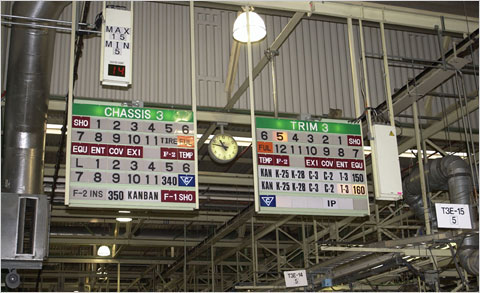
\includegraphics[scale=1.0]{figuras/kanbanindustria.png}
		\caption{Quadro Andon, com o mesmo objetivo do Kanban, na fábrica da Toyota \cite{kanbanindustria}}
\end{figure}

\section[Lean no Desenvolvimento de Software]{Lean no Desenvolvimento de Software}

\subsection[Abordagem]{Abordagem}

Mary e Tom Poppendieck fizeram um mapeamento dos princípios Lean na Manufatura em sete princípios em Lean no Desenvolvimento de software \cite{poppendieck}. Tais princípios serão detalhados nas seções a seguir. 

\subsection[Princípios]{Princípios}

\subsubsection[Eliminar o Desperdício]{Eliminar o Desperdício}

Eliminar desperdícios no sistema Lean de produção (manufatura) funciona da seguinte forma: olhar a linha do tempo desde a concepção do produto até a entrega ao cliente, e remover aquilo que não acrescenta valor (desperdícios). No desenvolvimento Lean de software o objetivo de eliminar desperdícos é o mesmo, porém, o início e  fim da linha do tempo podem ser alterados. A linha do tempo no desenvolvimento de software tem início no momento do pedido e para quando o pedido é entregue. Reduzir os desperdícios na linha do tempo significa reduzir a própria linha do tempo, ou seja, entregar o que foi pedido o mais rápido possível e com qualidade.

Para conseguir eliminar desperdícios é preciso, primeiramente, identificá-lo. Como desperdício é tudo que não agrega valor, é preciso ter conhecimento do que realmente é o valor. Na área de desenvolvimento de software, identicar o que é valor para o cliente é algo mais complexo, pois, dificilmente, no início do desenvolvimento o cliente sabe realmente o que quer, as suas necessidades e ou seus desejos mudam ao longo do desenvolvimento, alterando a definição do que agrega valor. No entanto, grandes organizações têm conseguido ter um conhecimento profundo do que é valor para o cliente e têm conseguido satisfazer suas necessidades. Assim, o objetivo de todas as organizações é conseguir alcançar esse entendimento profundo de valor.

A partir do momento que as pessoas conseguem identificar o que é valor, é possível começar a desenvolver a capacidade de identificar o que é desperdício. Qualquer atividade, não importante, que impeça o cliente de receber o que ele deseja e quando ele deseja é desperdício. Semelhante ao estoque no sistema produtivo, trabalhos inacabados no desenvolvimento de software gera todos os prejuízos com o fato de ser perdido, estar tecnologicamente atrasado, esconder problemas de qualidade e estagnar dinheiro.

Especificamente no desenvolvimento de software alguns desperdícios acontecem de forma constante: todos os requisistos especificados no início, que obviamente irão sofrer mudanças, testes realizados muito perto do fim, que claramente vão gerar muito retrabalho, e principalmente, funcionalidades desenvolvidas que nunca chegam a ser utilizadas.  De fato, estima-se que cerca de 20% das funcionalidades em um sisstema personalizado são regularmente usadas e cerca de dois terços delas são raramente usadas, o que gera custos desnecessários. 

\subsubsection[Integrar Qualidade]{Integrar Qualidade}

A meta dentro do desenvolvimento de software Lean é construir software com qualidade desde o início, não deixar para inserir testes só no final do de senvolvimento. A organização precisa ser bastante disciplinada. Para desenvolver um software com qualidade é preciso controlaras condições desde o começo de forma a não permitir defeitos. Como não é possível previnir todos os defeitos, é indicado inspecionar o produto após cada pequena funcionalidade ser implementada para que possa encontrar o defeito imediatamente após surgirem.

É importante ressaltar que o slogan “faça certo na primeira vez”, muito comumente usado, não se refere a construir o código e jamais modificá-lo, mas sim ao fato de usar-se as técnicas Test Driven Development (TDD), integração contínua e refatoração para garantir que um código simples e limpo que agregue valor ao cliente. 

\subsubsection[Criar Conhecimento]{Criar Conhecimento}

O desenvolvimento de software é um processo de criação do conhecimento.  Um processo de desenvolvimento concentrado em criar conhecimento esperará que o projeto evolua durante a codificação e não desperdiçará muito tempo fazendo todos os requisitos e arquitetura prematuramente. 

As empresas que já mostraram uma excelência a longo prazo em desenvolvimento de produtos compartilham um traço em comum: elas geram novo conhecimento por meio de uma experimentação disciplinada e codificam este conhecimento concisamente para torná-lo acessível ao restante da organização. Essas empresas não somente capturam dados explícitos, mas encontram maneiras de tornar explícito o conhecimento tático e fazê-lo parte da base de conhecimento organizacional (Referencia 16 da pag 53).

É importante ter um processo de desenvolvimento que encoraje o aprendizado sistemático durante todo o ciclo de desenvolvimento, mas também é preciso melhorar os processos de desenvolvimento. Às vezes, na constante busca por padrões ou modelos de processos, as empresas se prendem a uma documentação que torna mais difícil para as equipes de desenvolvimento melhorar diariamente seus próprios processos. Em Lean devem-se melhorar continuamente os processos, porque em ambientes complexos, sempre haverão problemas. 

A cada problema, é preciso acionar uma busca pela causa raiz, construir soluções possíveis para o problema e acionar uma mudança no processo para impedir que ele ressurja. Cada equipe de desenvolvimento deve reservar algum tempo para melhorar seus próprios processos.

\subsubsection[Adiar Comprometimentos]{Adiar Comprometimentos}

A ideia principal deste princípio é deixar as decisões irreversíveis para o último momento possível, ou seja, a última oportunidade de tomar a decisão antes que seja tarde demais, afinal de contas é um comprometimento que é tomado. Porém, isto não quer dizer que todas as decisões devam ser adiadas. Em primeiro lugar, é preciso tentar tornar a maioria das decisões reversíveis, ou seja, que possam ser mudadas ao decorrer do desenvolvimento sem prejuízos significativos. Um sistema de software não precisa ser completamente flexível, mas precisa que opções sejam preservadas em pontos onde as mudanças invariavelmente ocorram. É preciso experiência para saber quando devem ser mantidas essas opções.

\subsubsection[Entregar Rápido]{Entregar Rápido}

É a ideia deste principio é que é preciso entregar o software tão rápido que os clientes não tenham tempo de mudar de ideia.  As empresas que competem com base no tempo frequentemente têm uma vantagem significativa de custo sobre seus concorrentes. E para isso ser possível, elas eliminaram uma grande quantidade de desperdício, e desperdício tem influência diretamente no prazo e no custo. Além disso, velocidade repetível e confiável não é possível sem desenvolver com grande qualidade e, ainda, para ter sucesso tais empresas desenvolveram um profundo conhecimento sobre o que é valor para o cliente. Com a rapidez, é possível testar novas ideias e aprender o que funciona ou não funciona. 

\subsubsection[Respeitar as Pessoas]{Respeitar as Pessoas}

O princípio de respeitar as pessoas diz respeito a não impedir que as pessoas façam seus trabalhos só porque um outra pessoa acredita que não é a melhor forma de fazê-lo. Todos devem respeitar-se e trabalharem juntos na melhor solução. No processo de desenvolvimento também deve haver respeito, todos devem fazer parte da melhoria contínua dos processos. Existem três bases que sustentam o respeito às pessoas:

Líder empresarial: uma empresa que respeita as pessoas desenvolve bons líderes e garante que a equipe tenha o tipo de liderança que promove pessoas engajadas e pensantes, concentrando seus esforços na criação de um ótimo produto.

Mão de obra técnica especializada: empresas sábias garantem que a especialização técnica apropriada seja estimulada dentro da própria empresa e que as equipes estejam abastecidas da especialização necessária para atingir determinado objetivo.

Responsabilidade baseada em planejamento e controle: respeitar as pessoas significa que as equipes recebem planos genéricos e objetivos claros, e em vez de dizer como e o que fazer, desenvolve uma organização reflexiva onde as pessoas usam suas cabeças e descobrem isso sozinhas.

\subsubsection[Otimizar o Todo]{Otimizar o Todo}

Uma organização Lean otimiza todo o fluxo de valor, do momento em que recebe o pedido visando uma necessidade do cliente até o momento em que o software seja implantado e a necessidade do cliente seja atendida. Se houver concentração em otimizar apenas uma pequena parte do todo, inevitavelmente, o fluxo de valor completo sofrerá. 

\subsection[ Práticas]{ Práticas}

\subsubsection[Gerenciamento de Código Fonte e Scripts de Builds]{Gerenciamento de Código Fonte e Scripts de Builds}

O Gerenciamento de Código Fonte e Scripts de Builds não são práticas exclusivas do Lean, mas sim uma prática que deveria ser usada adotando Lean ou não, por isso é considerada como um pré-requisito para as práticas do Lean. Estas práticas ajudam a construir um time disciplinado e um ambiente de desenvolvimento estável.

O Gerenciamento de Código Fonte também é conhecido como controle de versão, basicamente, diz respeito a manter todo o código fonte e outros artefatos importantes do projeto em um repositório que mantém um histórico de versões de todos os itens de configuração, que são artefatos que precisam ser mantido sobre controle, pois sofrem mudanças e evoluções. Com o controle de versão é possível recuperar uma configuração, versão dos itens de configuração, em um momento desejado do tempo. Sempre é possível retornar a uma versão estável (baseline) quando erros são identificados.

O objetivo de realizar scripts de builds é automatizar todo o processo de construção do sistema e garantir que as mudanças no projeto são construídas, testadas e relatadas tão logo quanto o possível depois de serem relatadas. Como resultado, o build do sistema é gerado da mesma forma em todas as vezes. Esta prática elimina erros escondidos e torna mais fácil a inserção de novos integrantes à equipe. E também torna mais fácil realizar testes e a entrega de release do software, uma vez que constrói arquivos executáveis e de instalação do produto \cite{hibbs2009}.

\subsubsection[Teste Automatizado]{Teste Automatizado}

Um sistema à prova de erros é uma das práticas fundamentais do Lean. É parte central da produção de um produto com qualidade e da redução de desperdícios. O teste automatizado é um dos principais meios de evitar erros no desenvolvimento de software. O teste automatizado engloba todos os tipos de testes: teste unitário, teste de integração, teste de aceitação, teste de desempenho, teste de carga, desenvolvimento orientado a testes, etc.

Cada um dos tipos de testes possui um objetivo principal, mas todos eles têm os seguintes objetivos em comum:
\begin{itemize}
\item Os testes são criados manualmente pelos desenvolvedores.
\item Todos os testes podem ser executados automaticamente, sem intervenção humana.
\item Os erros são detectados automaticamente.
\item O desenvolvedor é notificado quando os erros acontecem.
\end{itemize}

O teste automatizado suporta três princípios do Lean: eliminação de desperdícios, qualidade na raiz e criar conhecimento. Ele ajuda a eliminar desperdícios que geram retrabalho e custos quando erros são detectados apenas nas fases finais do ciclo de desenvolvimento de software. No que diz respeito a construir com qualidade, o teste automatizado é um dos principais meios. Uma base de código com uma suíte de testes automatizados realiza a validação e checagem de forma automática, o que reduz a possibilidade de erros não detectados seja introduzido dentro do software.

Além disso, os testes automatizados servem como uma documentação atualizada do que está sendo feito. Ele cria um conhecimento primário e confiável para os desenvolvedores porque garante conformidade com o esperado toda vez que a suíte de teste é executada com sucesso \cite{hibbs2009}.

\subsubsection[Integração Contínua]{Integração Contínua}

A integração diz respeito ao momento que todos os módulos ou componentes do software que está sendo desenvolvido são executados juntos. Componentes individuais, banco de dados, interfaces de usuário e recursos do sistema são todos reunidos e testados em cima da arquitetura. A integração envolve verificar a comunicação dos componentes e garantir que a mensagem passada entre eles é compatível e completa. 

O processo de desenvolvimento tradicional trata integração como uma fase separada que ocorre depois que todos os componentes tenham sido implementados, o que costuma gerar uma serie de correções e retrabalho. A integração contínua transforma a tradicional fase de integração em uma atividade que ocorre durante toda o processo de implementação do sistema.

A integração contínua é o processo de integrar pequenas mudanças em uma base estável para entrega de um novo release do produto. Integrando pequenas mudanças em um curto intervalo, os desenvolvedores podem evoluir o produto um pouco de cada vez enquanto garantem que cada novo pedaço funciona corretamente com todo o resto do sistema. A integração contínua usa testes unitários para garantir que cada pequena parte do sistema está implementada corretamente e usa o gerenciamento do código fonte e os scripts de build para garantir que a cada nova pequena integração nada foi quebrado, ou seja, garantir que o sistema continue funcionando corretamente como um todo \cite{hibbs2009}. 

\subsubsection[Menos Código ]{Menos Código}

A prática de escrever menos código não diz respeito a escrever menos software, mas sim a ter todas as funcionalidades implementadas com poucas linhas de código e de maneira simples. Diz respeito a eliminar código desnecessário e fazer com que o código necessário se torne mais eficiente, mantendo a base de código pequena ao menos tempo em que funcionalidades (valor) são entregues ao cliente.

O tamanho da base de código afeta o projeto de vários modos. Quanto maior o código maior é a quantidade de componentes que precisam ser conectadas e mais esforço de integração será gasto. Quanto maior o tamanho da base de código mais erros podem ser gerados e mais esforço para encontrar e corrigir os erros será gasto. Ainda, quanto maior o tamanho maior é a dificuldade de entender o que foi desenvolvido, aumentando a curva de aprendizado de novos desenvolvedores e futuros mantedores.  

Como uma base de código grande acarreta em mais componentes, mais bugs e grande curva de aprendizagem, como consequência terá mais custos em desenvolvimento e manutenção. A definição de desperdício no desenvolvimento Lean é qualquer coisa que aumente os custos sem produzir valor, então o custo de desenvolvimento e manutenção resultante de uma grande base de código pode ser considerado como desperdício. 

Para escrever menos código e manter o valor desejado pelo cliente, os desenvolvedores precisam adotar uma atitude de olhar criticamente para cada linha de código. Minimizar o tamanho do código, no entanto, não é limitar a implementação. Os desenvolvedores precisam ser minimalistas durante todo o processo de desenvolvimento, desenvolvendo de maneira simples cada funcionalidade. Um design simplista facilita, ainda, a implementação de mudanças \cite{hibbs2009}. Os padrões e técnicas podem ser utilizados para auxiliar os desenvolvedores a desenvolver apenas o código que é realmente necessário, por exemplo, utilizar padrões de design, reuso e refatoração.

\subsubsection[Iterações Curtas]{Iterações Curtas}

O desenvolvimento iterativo entrega software funcional ao cliente para avaliação a cada intervalo específico de tempo. Cada iteração adiciona novas funcionalidades ao produto e aumenta o entendimento do cliente sobre como o produto final irá atender à suas necessidades. A efetividade do processo iterativo vem da oportunidade de ter o feedback do cliente e incorporar esse feedback ao desenvolvimento. O feedback do cliente é que irá direcionar a próxima iteração quanto a adição, remoção ou modificação de requisitos e implementação. Quanto menor a iteração, mais oportunidades de receber o feedback do cliente e maior é a possibilidade de atender o que o cliente deseja no produto final. 

As iterações curtas suportam três princípios do Lean: eliminar desperdício, adiar compromisso e entrega rápida. Existem duas formas de desperdícios advindos de iterações largas, o trabalho parcial, aquele que não é construído de forma completa seja com requisitos não implementados ou incompletos quanto com código não testado, porque não adiciona novo valor ao produto e o replanejamento, quando o planejamento inicial é feito para um futuro muito distante e as necessidades e desejos do cliente podem mudar fazendo com que seja preciso o realizar o replanejamento, porque o trabalho planejado anteriormente é desperdiçado. As iterações curtas previnem tais situações de desperdícios, pois o esforço fica concentrado em desenvolver o que é de alta prioridade para o cliente mais rapidamente e planeja tão longe quanto necessário para manter o desenvolvimento.  

O princípio de adiar compromisso, como já explicado anteriormente, diz respeito a adiar decisões importantes tanto quanto possível. Adiar tais decisões fornece aos desenvolvedores tempo para coletar e entender as informações necessárias para o desenvolvimento, e iterações curtas dão oportunidades de coletar informações por meio do feedback do cliente. Os desenvolvedores podem criar protótipos do produto final já nas iterações iniciais, recebem o feedback e usam o feedback para decidir a implementação final nas iterações finais \cite{hibbs2009}.

As iterações curtas, claramente, suportam o princípio de entrega rápida devido a redução dos intervalos de contato com o cliente e por entregar novas funcionalidades rapidamente para receber feedback. Em vez de esperar até o final do desenvolvimento para vê os efeitos das suas solicitações, o cliente já poderá visualizá-los na próxima iteração. 

\subsubsection[Participação do Cliente]{Participação do Cliente}

Se o objetivo do desenvolvimento de um produto é criar um produto que o cliente irá usar, é importante ter a participação do cliente em grande parte do processo. Os conceitos de priorizar requisitos e de realizar correções de acordo com o feedback do cliente necessitam de participação ativa do cliente no processo de desenvolvimento. 
Os clientes são as melhores fontes de informações sobre o domínio do problema.  Eles sabem as atividades que precisam ser feitas, eles sabem as condições que o software será executado e eles sabem os objetivos que desejam atingir com a solução. No entanto, eles raramente sabem sobre a tecnologia que será usada na implementação da solução.  

Por outro lado, os desenvolvedores sabem sobre as a tecnologias e sabem o caminho mais eficiente para modelar e implementar problemas e soluções. O que os desenvolvedores não sabem é sobre os conhecimentos do negócio no qual a solução será incorporada. 

Combinando o conhecimento do negócio do cliente com o conhecimento técnico do desenvolvedor cria uma equipe dinâmica que resulta em um desenvolvimento de um melhor produto. Desenvolvedor e clientes trabalhando juntos inspiram um ao outro a criar algo melhor do que eles poderiam criar individualmente \cite{hibbs2009}.


\subsubsection[Kanban]{Kanban}

O Kanban no desenvolvimento de software surgiu a partir do Kanban do Lean na manufatura, ambos usam um mecanismo de controle visual para acompanhar o trabalho à medida que ele flui através das várias etapas do fluxo de valor. 

\begin{figure}[h]
		\centering
		\label{fig05}
			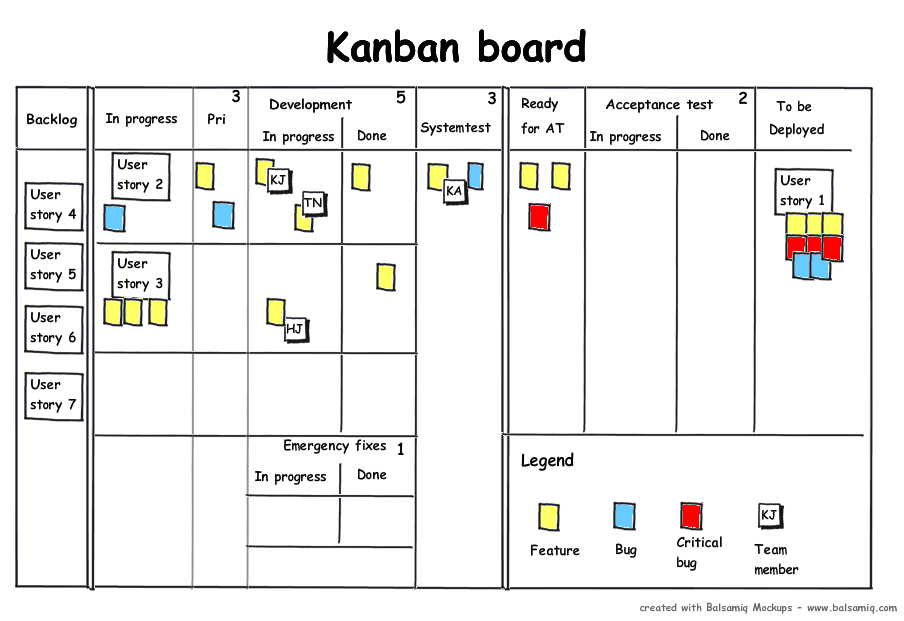
\includegraphics[scale=0.7]{figuras/kanban.png}
		\caption{Quadro Kanban \cite{kanban}}
\end{figure}

O Kanban não é um processo ou ciclo de vida de gerenciamento de projetos ou de desenvolvimento de software. Ele é uma abordagem para introduzir mudanças em um ciclo de desenvolvimento de software ou metodologia de gerenciamento de projetos. O Kanban tem três conceitos básicos: visualizar o fluxo de trabalho, limitar o trabalho em progresso (WIP – work in progress) e medir e melhorar o fluxo. 

Para visualizar o fluxo de trabalho divida o trabalho em partes, escreva cada item em um cartão, ou post-its, e coloque no quadro Kanban, e use colunas nomeadas para ilustrar onde cada item está no fluxo de trabalho. Com o mapeamento do fluxo de trabalho já é possível ter o entendimento do processo atual. 
Para limitar o WIP é preciso associar limites explícitos para quantos itens podem estar em progresso em cada estado do fluxo de trabalho, existe um número limite de tarefas que podem ser bem feitas durante um mesmo período de tempo. É preciso saber também a diferença entre a complexidade das tarefas, duas tarefas podem ser feitas em uma semana assim como duas tarefas podem ser feitas em três horas, tudo dependerá de quanto esforço será gasto em cada uma. As métricas do Kanban ajudam a chegar a um número ótimo.

\begin{figure}[h]
		\centering
		\label{fig05}
			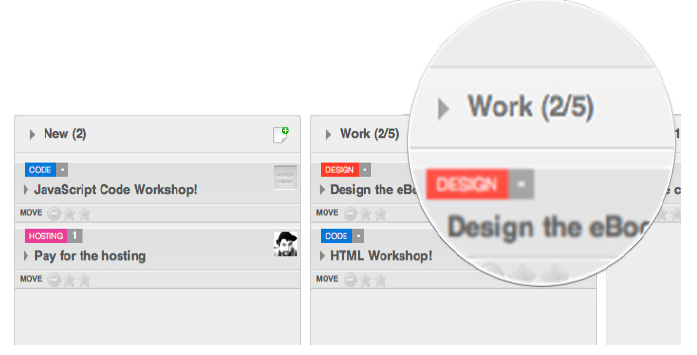
\includegraphics[scale=0.5]{figuras/WIP.png}
		\caption{Work in Progress  \cite{klipp}}
\end{figure}


Além disso, com o WIP limitado em um sistema Kanban, tudo que fica bloqueado por qualquer motivo tende a parar o sistema. Se certa quantidade de itens de trabalho fica bloqueada, todo o processo para de funcionar. Isso cria a necessidade de concentrar toda a equipe e toda a empresa na solução do problema para desbloquear o item e restaurar o fluxo. 

A melhoria deve sempre ser baseada em objetivos mensuráveis, e no Kanban isto não é diferente. Encontrar e aplicar boas métricas é geralmente um passo difícil,  mas algumas métricas simples automaticamente geradas por uma aplicação pode dar a informação necessária para otimizar o processo e maximizar a eficiência \cite{klipp}. 

\begin{figure}[h]
		\centering
		\label{fig05}
			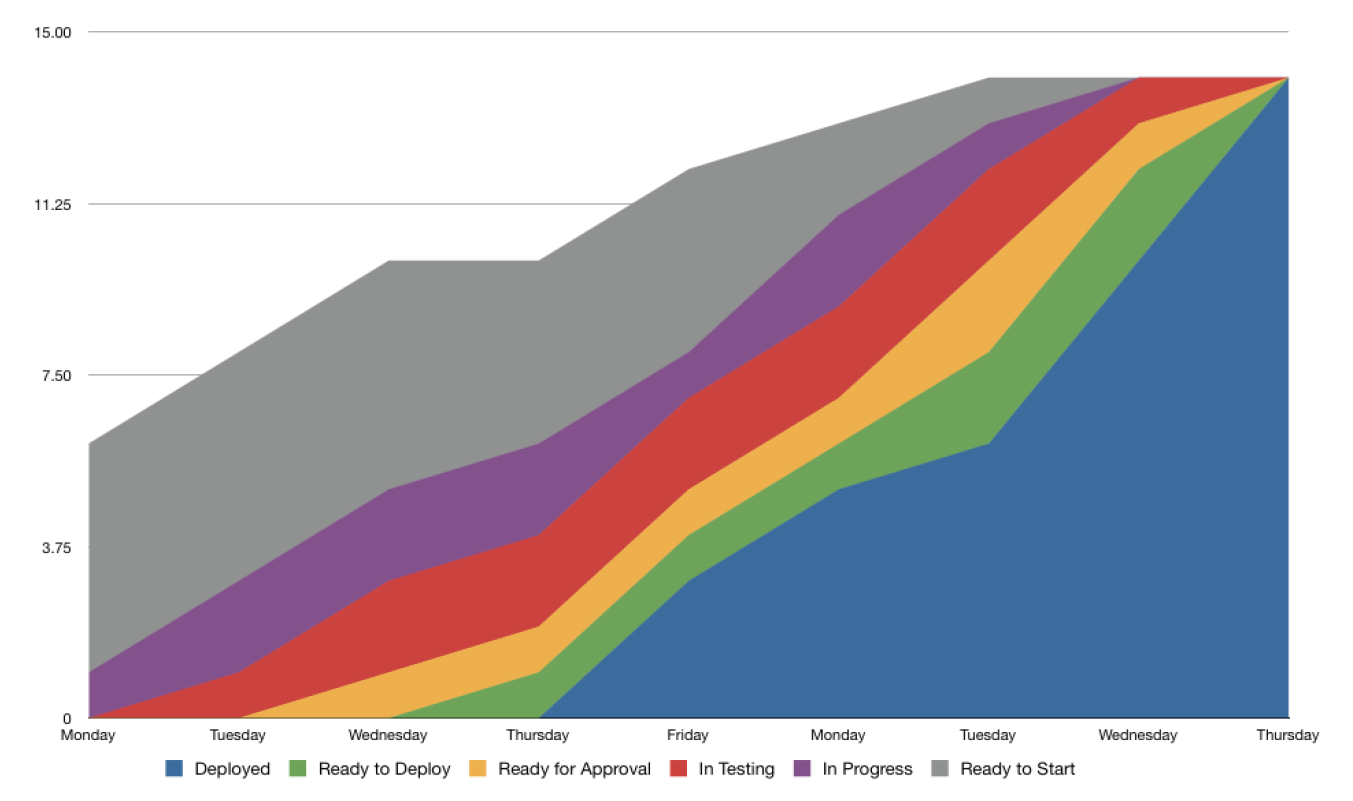
\includegraphics[scale=0.4]{figuras/metricasKanban.png}
		\caption{Gráfico de Medições Kanban  \cite{klipp}}
\end{figure}

O Kanban, no entanto, vai um passo além e dá transparência ao processo e seu fluxo. O Kanban expõe gargalos, filas, variabilidade e desperdício. Tudo que impacta o desempenho da organização em termos de quantidade de trabalho de valor entregue e o tempo de ciclo necessário para entregá-lo. Proporciona aos membros da equipe e às partes interessadas externas a visibilidade sobre os efeitos de suas ações (ou falta de ações) e esta visibilidade incentiva a discussão sobre melhorias que precisam ser feitas nos seus processos encorajando a evolução incremental dos processos existentes. Ainda, o  Kanban, através da natureza do sistema pull, encoraja também comprometimento tardio, tanto em priorização de trabalho novo quanto na entrega de trabalho existente \cite{kniberg2009}. 
